% 用 xelatex 编译, 推荐配方 xe->bib->xe->xe
\documentclass[12pt,a4paper,UTF8]{ctexart}
% 基础宏包
\usepackage{geometry} % 页面设置
\usepackage{setspace} % 行距设置
\usepackage{titlesec} % 标题格式
\usepackage{titletoc} % 目录格式
\usepackage{graphicx} % 插图
\usepackage{float}    % 浮动体, 设置图片位置
\usepackage{booktabs} % 表格美化
\usepackage{amsmath,amssymb,mathrsfs} % 公式
\usepackage{fancyhdr} % 页眉页脚
\usepackage{enumitem} % 列表
\usepackage{footnote} % 脚注
\usepackage{lastpage} % 最后一页页码
\usepackage{fontspec} % 英文字体设置
\usepackage{amsthm,thmtools,thmbox} % 数学定理

% tikz 作画相关宏包
\usepackage{tikz} % tikz 作图
\usepackage{pgf} % tikz 中使用公式作画
\usepackage{tikz-cd} % tikz 绘制交换图的宏包
\usepackage{caption} % 标题

% 基于毕业论文要求的一些特殊设定宏包
\usepackage{gbt7714} % GBT-7714 引用标准
\bibliographystyle{gbt7714-numerical} % 按数字来索引
\usepackage{pdfpages} % 插入PDF文件
\usepackage{indentfirst} % 强制首行缩进

% 批注
\usepackage[markup=default,draft]{changes} % 批注, draft 表示显示批注, 换成 final 隐藏批注

% 超链接
\usepackage{hyperref} % 超链接（最后加载避免冲突）

% 页面设置：左3.17cm，右3.17cm，上2.54cm，下2.54cm，页眉1.5cm，页脚1.75cm
\geometry{
  left=3.17cm,
  right=3.17cm,
  top=2.54cm,
  bottom=2.54cm,
  headheight=1.5cm,
  footskip=1.75cm
  }

% 字体设置：通过ctex自带命令设置，避免fontspec冲突
\setCJKmainfont{SimSun}       % 中文主字体(宋体)
\setCJKsansfont{Microsoft YaHei} % 中文无衬线字体
\setmainfont{Times New Roman} % 英文主字体

% 全局段落与行距配置（核心修复：先设置缩进，再设置行距，保证优先级）
\setlength{\parindent}{2em}        % 全局首行缩进2字符（优先设置）
\setlength{\parskip}{0pt}          % 段间距0
\doublespacing

% 页码设置：前期罗马数字，正文阿拉伯数字，底端居中，小五号
\pagestyle{plain}
\fancyhf{}
\cfoot{\thepage}
\renewcommand{\footrulewidth}{0pt}
\renewcommand{\thepage}{\roman{page}} % 初始罗马数字

% 一级标题：黑体三号，居中，单倍行距
\titleformat{\section}
  {\bfseries\Large\heiti\centering}{\thesection}{0.5em}{}
\titlespacing*{\section}{0pt}{12pt}{6pt}

% 二级标题：黑体小三号，左对齐，单倍行距
\titleformat{\subsection}
  {\bfseries\large\heiti}{\thesubsection}{0.5em}{}
\titlespacing*{\subsection}{0pt}{12pt}{6pt}

% 三级标题：黑体四号，左缩进0.85cm，单倍行距
\titleformat{\subsubsection}
  {\bfseries\normalsize\heiti}{\thesubsubsection}{0.5em}{}
\titlespacing*{\subsubsection}{0.85cm}{12pt}{6pt}

% 目录格式与 word 模板相匹配, 调整了缩进量和取消 section 标题的加粗 
\titlecontents{section}[0em]{\CJKfamily{sun}}{\normalfont\thecontentslabel\quad}{}{\titlerule*[6pt]{.}\contentspage}
\titlecontents{subsection}[1em]{\CJKfamily{sun}}{\normalfont\thecontentslabel\quad}{}{\titlerule*[6pt]{.}\contentspage}
\titlecontents{subsubsection}[2em]{\CJKfamily{sun}}{\normalfont\thecontentslabel\quad}{}{\titlerule*[6pt]{.}\contentspage}

% 图表公式编号：连续编号
\renewcommand{\thefigure}{\arabic{figure}} % 图阿拉伯数字连续编号
\renewcommand{\thetable}{\arabic{table}}   % 表阿拉伯数字连续编号
\renewcommand{\theequation}{\arabic{equation}} % 公式阿拉伯数字连续编号

% 引用时区分上标和普通大小
\let\oldcite\cite % 保存老cite
\renewcommand{\cite}[1]{%
  \citestyle{numbers}% 每次引用前执行该指令，调整为正常大小
  \oldcite{#1}% 调用原有\cite功能，传递参数#1
}
% 设置新命令 \upcite{}
\newcommand{\upcite}[1]{%
  \citestyle{super}% 每次引用前执行该指令，调整为上标
  \oldcite{#1}% 调用原有\cite功能，传递参数#1
}

% 参考文献格式：仿宋体五号，1.5倍行距，悬挂缩进
\newcommand{\refstyle}{\CJKfamily{fangsong}\small\onehalfspacing\setlength{\parindent}{0em}\setlength{\hangindent}{0.74cm}}

% 附录格式：仿宋体五号，1.5倍行距，首行缩进2字符
\newcommand{\appendixstyle}{\CJKfamily{fangsong}\small\onehalfspacing\setlength{\parindent}{2em}}

% 自定义样式

\let\example\undefined % 宏包自带了例子环境, 我们首先需要将其无效化, 才能使用我们的环境
\let\endexample\undefined

\declaretheoremstyle[
  name=\hspace{2em}% 参考部分研究生毕业论文, 定理/定义等环境前加入首行缩进 \hspace{2em}, 可去除
  定理, 
  bodyfont=\normalfont,
  headfont=\bfseries\heiti,
  postheadspace=0.5em,
  spaceabove=1.5pt,
  spacebelow=1.5pt,
  %headpunct={: },    % 标题后加中文冒号 (可选, 适配中文排版) 
  within=section % 按章节划分序号
]{thmsty}
\declaretheorem[style=thmsty]{theorem}

% 其他环境的设置
\declaretheoremstyle[
  name=\hspace{2em}% 参考部分研究生毕业论文, 定理/定义等环境前加入首行缩进 \hspace{2em}, 可去除
  引理,
  bodyfont=\normalfont,
  headfont=\bfseries\heiti,
  postheadspace=0.5em,
  spaceabove=1.5pt,
  spacebelow=1.5pt,    % 取消定理下方额外间距
  %headpunct={: },    % 标题后加中文冒号 (可选, 适配中文排版) 
  within=section       % 按章节编号 (如1.1 引理1) , 可选
]{lemsty}
\declaretheorem[style=lemsty,sibling=theorem]{lemma} % 沿用定理环境的编号

\declaretheoremstyle[
  name=\hspace{2em}% 参考部分研究生毕业论文, 定理/定义等环境前加入首行缩进 \hspace{2em}, 可去除
  例, % 可以考虑是选择 例 还是 例子
  bodyfont=\normalfont,
  headfont=\bfseries\heiti,
    spaceabove=1.5pt,
  spacebelow=1.5pt,
  postheadspace=0.5em,
  within=section
]{exsty}
\declaretheorem[style=exsty,sibling=theorem]{example} % 统一编号顺序

\declaretheoremstyle[
  name=\hspace{2em}% 参考部分研究生毕业论文, 定理/定义等环境前加入首行缩进 \hspace{2em}, 可去除
  定义,
  bodyfont=\normalfont,
  headfont=\bfseries\heiti,
    spaceabove=1.5pt,
  spacebelow=1.5pt,
  postheadspace=0.5em,
  within=section
]{defsty}
\declaretheorem[style=defsty,sibling=theorem]{definition} % 统一编号顺序

\declaretheoremstyle[
  name=\hspace{2em}% 参考部分研究生毕业论文, 定理/定义等环境前加入首行缩进 \hspace{2em}, 可去除
  注记,
  bodyfont=\normalfont,
  headfont=\bfseries\heiti,
    spaceabove=1.5pt,
  spacebelow=1.5pt,
  postheadspace=0.5em,
  within=section
]{rmksty}
\declaretheorem[style=rmksty,sibling=theorem]{remark} % 统一编号顺序

\declaretheoremstyle[
  name=\hspace{2em}% 参考部分研究生毕业论文, 定理/定义等环境前加入首行缩进 \hspace{2em}, 可去除
  推论,
  bodyfont=\normalfont,
  headfont=\bfseries\heiti,
    spaceabove=1.5pt,
  spacebelow=1.5pt,
  postheadspace=0.5em,
  within=section
]{corsty}
\declaretheorem[style=corsty,sibling=theorem]{corollary} % 统一编号顺序

\declaretheoremstyle[
  name=\hspace{2em}% 参考部分研究生毕业论文, 定理/定义等环境前加入首行缩进 \hspace{2em}, 可去除
  命题,
  bodyfont=\normalfont,
  headfont=\bfseries\heiti,
    spaceabove=1.5pt,
  spacebelow=1.5pt,
  postheadspace=0.5em,
  within=section
]{propsty}
\declaretheorem[style=propsty,sibling=theorem]{proposition} % 统一编号顺序

% 证明环境
\makeatletter
\renewenvironment{proof}[1][\proofname]{% 保留可选参数（默认“证明”）
  \par
  \pushQED{\qed}% 保留证明结尾的QED符号
  \topsep6\p@\@plus6\p@\relax  % 原生上下间距
  \trivlist
  \item[\hskip\labelsep\hspace{2em}\bfseries\heiti #1]\ignorespaces  % 缩进 2 字符
}{%
  \popQED\endtrivlist\@endpefalse
}
\makeatother

% 列表设置
\setlist{
  itemsep=0pt,         % 列表项之间的间距
  parsep=0pt,          % 段落之间的间距
  topsep=0.5ex,        % 列表与上下文距离（可微调）
  partopsep=0pt,
  leftmargin=*,        % 保持正常缩进
  align=left,
}

% 在这里定义你自己的符号, 适用那些用 \mathrm{} 的符号
\DeclareMathOperator{\Spec}{Spec}



\begin{document}
\pagestyle{empty} % 封面、诚信声明无页码

% ===================== 封面 =====================
% 插入封面的 PDF 文件, 记得先用 word 修改之后导出为 PDF 文件并放在目录下面
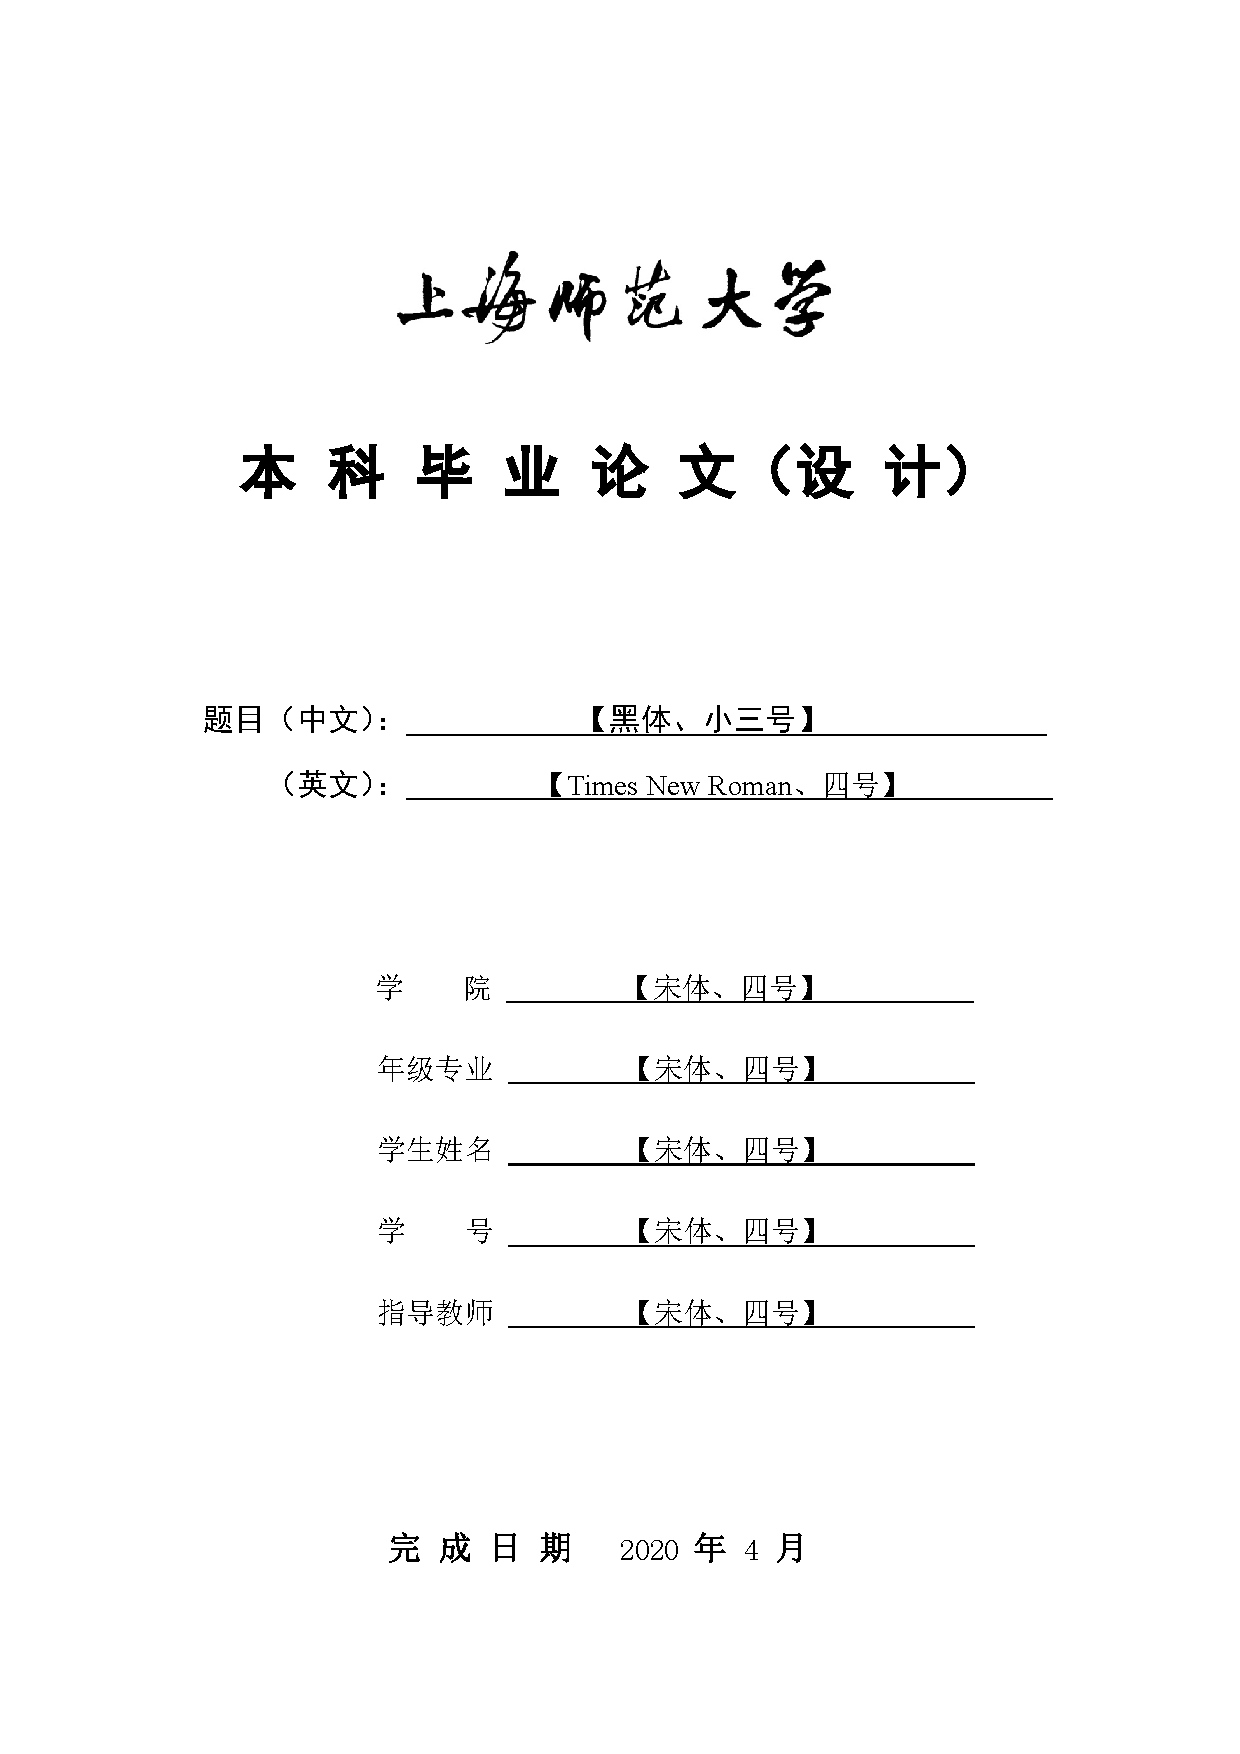
\includepdf[pages=-, scale=1]{本科毕业论文封面 - 已改.pdf} 

\newpage

% ===================== 诚信声明 =====================
% 插入诚信声明的 PDF 文件, 记得先用 word 修改之后导出为 PDF 文件并放在目录下面

\includepdf[pages=-, scale=1]{本科毕业论文诚信声明 - 已改.pdf}
\newpage

% ===================== 中文摘要与关键词 =====================
\begin{center}
\textbf{\Large\heiti 摘要}
\end{center}
% 修复：先设置固定行距，再恢复首行缩进（用\par保证段落生效）
\singlespacing
\setlength{\baselineskip}{20pt} % 固定值20磅
\CJKfamily{sun}\normalsize % 确保宋体生效
% 摘要正文（首行缩进2字符）
\hspace{2em}
本文以XX为研究对象，采用XX研究方法，探讨了XX问题，分析了XX原因，得出了XX结论，为XX提供了参考依据。\par
\vspace{1em}
\noindent\textbf{\heiti 关键词：}
\CJKfamily{sun}\normalsize 代数几何; 微分几何; 算术几何

\quad 


% 如果中文摘要和英文摘要内容不多, 可以在一面呈现, 就将下面的 \newpage 前加上 % 
\newpage

% ===================== 英文摘要与关键词 =====================
\begin{center}
\textbf{\Large Abstract}
\end{center}
\singlespacing
\setlength{\baselineskip}{20pt} % 固定值20磅
\normalsize
% 摘要正文（首行缩进2字符）
\hspace{2em}
This thesis takes XX as the research object, adopts XX research methods, discusses XX issues, analyzes XX causes, draws XX conclusions, and provides a reference for XX.\par
\vspace{1em}
\noindent\textbf{Keywords:} Algebraic geometry; differential geometry; arithmetic geometry
\vspace{2em}
\newpage

% ===================== 目录 =====================

\singlespacing
\setlength{\baselineskip}{20pt} % 固定值20磅

\vspace{1em}
\tableofcontents
\vspace{2em}
\newpage

% 正文开始，页码改为阿拉伯数字
\pagestyle{plain}  % 启用基础页码样式（页码在页脚居中）
\renewcommand{\thepage}{\arabic{page}}
\setcounter{page}{1}

\singlespacing
\setlength{\baselineskip}{20pt} % 固定值20磅

% ===================== 正文 =====================
% 1 导言
\section{导言}

数学论文, 特别是基础数学的论文, 一般的编排顺序是导言、预备知识, 
接着再是正文内容. 为了让模板更加好用, 我们在导言部分和预备知识部分
只展示大致的编排样式, 进入正文部分再展开详细的教学. 

\subsection{研究背景与意义}

数学相关论文的研究背景与意义通常是比较好写的, 可以参考国内外论文和专著的导言
部分, 一般前沿的文章在这一部分都写得相当出色, 能够让大部分读者一下子抓住要点. 
不过论文和专著的特性也决定了它们所需的知识储备往往远远超出本科生能力范围, 
因此一些受众更加广泛门槛更加低的文章会是更适合本科生的学习资源. 
在此我推荐一部分可以找到这类文章的期刊/平台: 
\begin{itemize} % 使用 itemize 环境来表示无序号的条目
  \item \href{https://www.ams.org/notices}{\textbf{Notices of the American Mathematical Society}}: 
  \begin{itemize}[label = $ \circ $] % 这里使用了 enumitem 宏包中的功能, 可以自定义 item 的标志
    \item 这本期刊并非传统的原创研究期刊, 而更像是一本面向全球专业数学家的综合性新闻杂志, 
    里面的文章往往用较少的篇幅深入浅出地讲解一些数学方向的前沿发展. 

    \item 在这本期刊上, 数学工作者们会向研究生和其他数学工作者解释自己在做什么工作, 
    例如许晨阳介绍 $ K $-稳定性进展的文章 \cite{Xu2022} 
    和王艺霖介绍她所研究的随机几何相关的文章 \cite{Wang2024}; 
    许多文章也会从一些有趣又不至于晦涩的内容出发, 来介绍前沿的理论, 
    例如陶哲轩的 \cite{Tao2001} 从挂谷猜想出发来讨论分析和组合工具在这一类问题中的应用; 
    此外, 像 \cite{Dickenstein2020} 这样的将看似不相干的两个领域 
    (代数几何和生物学) 相交叉结合的内容对于诸多数学工作者都是相当有看头的. 

    \item 推荐的另一个理由是里面有很多精美的插图, 我在答辩时就曾使用 \cite{Alper2025} 
    中的一些图片. 
  \end{itemize}
  
  \item \href{https://pubs.ams.org/BULL/}{\textbf{Bulletin of the American Mathematical Society}} 
  \& \href{https://www.lms.ac.uk/publications/blms}{\textbf{Bulletin of the London Mathematical Society}}: 

  \begin{itemize}[label = $ \circ $] % 这里使用了 enumitem 宏包中的功能, 可以自定义 item 的标志
    比起 Notices Amer. Math. Soc. 这两本期刊的专业性更强, 
    是经典的综述性学术期刊, 文章的篇幅更长, 内容更加详实, 有些文章都堪称
    某一方向的入门手册. 
    
    下面我们以一些文章为代表来了解一下这两部期刊. 

    \item 无理数和超越数 (即不是任何多项式的零点的复数) 的判别一直是一个复杂的问题, 
      $ \pi $ 的无理性的第一次证明是 1761 年由 Lambert 用连分数给出的, 
      2026 年丘成桐大学生数学竞赛分析与微分方程赛道第一题也有关于 $ \pi $ 
      的无理性, 其中积分 $ I_{n} $ 的构造可以视作 Siegel 的构造的一种变形 
      (参考知乎回答: \href{https://www.zhihu.com/question/2038923497062261595/answer/2040190430910862250}
      {如何评价2026年丘成桐大学生数学竞赛? - 万物皆数数海拾贝的回答 - 知乎}), 
      而 $ \pi $ 是无理数的最简单的一个证明是 Niven 在 \cite{Niven1947} 
      里面给出的, 只需要简单的数学分析知识就足矣完成这个证明. 

    \item Euler 常数 $ \gamma = \lim\limits_{n \to \infty} \left( \sum\limits_{i=1}^{n} \dfrac{1}{i} - \ln n \right) $ 
      是数学分析的经典例子, 但关于它是否是超越数仍然是一个开放的问题, 
      \cite{Lagarias2013} 展示了 $ \gamma $ 常数的历史与现代的研究进展, 
      以及它是如何与许多数论问题相联系起来的. 

    \item Hermite 矩阵是高等代数里常见的对象, 其对角线和特征值皆为实数. 
      Schur-Horn 定理指出 Hermite 矩阵的对角元与特征值的某种关系, 这种关系可以被描述为
      对角线向量位于所有特征值向量 (特征值的任意排列构成的向量) 的凸包之中. 
      Atiyah \cite{Atiyah1982} 将这种凸性现象推广至辛流形和 K\"{a}hler 流形
      上, 给出了 Schur-Horn 定理的几何表述. 

    \item 上面谈论了数学分析和高等代数, 现在我们把高度稍微拔高, 来到抽象代数的领域. 
      代数学有一个亘古不变的使命: 分析出一系列数学对象的代数结构, 并给出其分类, 
      作为最基本的代数结构之一, 群的分类问题是代数学家一直关心的. 
      根据 Jordan-H\"{o}lder 定理, 任意有限群都有合成群列并且唯一, 
      其中有限单群作为合成群列的骨架, 其分类是有限群分类的根基. 
      有限单群的分类定理的证明涉及约 100 位作者在 500 篇期刊文章中完成的超万页文献, 
      最终于 2004 年通过补漏洞得以完善, 是上个世纪数学界的一项壮举. 
      这一定理指出, 有限单群可以分类为素数阶循环群 $ \mathbb{Z} / p \mathbb{Z} $、
      交错群 $ A_{n} $ ($ n\geq 5 $)、16 族 Lie 型单群以及 26 个散在单群. 
      在这些散在单群中, 魔群是最为特殊的一个, 它的阶数达到了约 $ 8 \times 10^{53} $, 
      其最小的忠实复表示的维数也达到了 196883. 
      1978 年, McKay 察觉了这些庞大的数字背后的奥秘, 他在研究模函数的 $ j $-函数
      的展开式时, 发现一次项系数为 196884, 并且这些系数都可以分解为魔群不可约表示的
      维数的线性组合. McKay 将他的发现告诉 Conway, Conway 认为魔群与模形式之间的这种联系
      是某种酒鬼胡话 (moonshine 的隐喻), 并在与 Norton 合作的文章 \cite{ConwayNorton1979} 
      中将这一联系命名为月光猜想 (moonshine conjecture), 
      这一文章的题目则叫做魔群月光 (Monstrous Moonshine), 
      或许是最浪漫的数学术语, 更浪漫的是, 
      Borcherds \cite{Borcherds1992} 在 1992 年使用弦论和顶点算子代数的技术证明了
      月光猜想. 
  \end{itemize}

  \item \href{https://pubs.ams.org/ebooks/pspum}{\textbf{Proceedings of Symposia in Pure Mathematics}}: 
  \begin{itemize}[label = $ \circ $]
    \item \cite{Knapp1997}
    \item \cite{Brion2017}
    \item \cite{delaLlave2001}
    \item \cite{Totaro1999}
    \item \cite{Scholl1994}
    \item \cite{DonagiWitten2015}
  \end{itemize}
  
  

  \item \href{https://www.sciencedirect.com/journal/expositiones-mathematicae}{\textbf{Expositiones Mathematicae}}: 
  这是专门收录数学综述的期刊, 但诚如 \href{https://mathoverflow.net/questions/15366/which-journals-publish-expository-work/15369#15369}{
  Timothy Chow 在这个评论下的回答}, 它最大的缺点就是知名度太低以至于很多
  优秀的综述文章并未将其当作第一选择. \cite{Olsen&Holden2010}
\end{itemize}

\subsection{国内外研究现状}

在这里我们就要大量引用文献了, 本模板仿照中文 word 论文模板标准, 采用两种引用形式. 

\begin{itemize}
  \item 第一种, 当这篇文献直接当主语或者宾语时, 直接用正体形式. 例如: 
  实际上, 模空间最早的研究起源于黎曼在 1857 年关于 Abel 函数的论文 \cite{Riemann1857}, 
  他在这篇文章中提出了黎曼曲面的定义, 并通过研究亏格为 $g$ 的曲线所构成的空间提出了 
  "参数" 空间的想法. 中文早期对 "moduli space" 的翻译 "参模空间" 就是源自于模空间
  中参数化的思想. 

  \item 第二种, 当我们引用这篇文献的内容需要指出该内容的出处时, 采用上标形式. 例如: 
  在埃尔朗根纲领的指导下, 几何的研究已经与几何对象的变换群的研究脱不开关系了. 
  因此经典不变量理论在 19 世纪有相当多的发展, 其中希尔伯特经典的 23 个问题中的第 14 个, 
  即有限生成的 $k$-代数在代数群作用下的不变环是否是有限生成的, 就是围绕这一问题展开. 
  很遗憾, 希尔伯特的猜想最终被证明是错误的 \upcite{Nagata1959}. 
\end{itemize}


\subsection{研究内容}

这里讲讲你的论文里干了什么

% 第二章 预备知识

\section{预备知识}



\subsection{范畴论基础}

\subsubsection{米田引理与可表函子}

先回顾一下函子的概念, 以及代数几何中无处不在的函子性, 最后点出一般的预层
的反变函子定义 (与后面的无法构建模空间的反例对应)

首先讲一下米田引理的哲学

\begin{definition}[可表函子]
  设 $\mathcal{C}$ 为一个范畴, $X \in \mathcal{C}$ 为一个固定的对象, 
  点函子 $h_X : \mathcal{C} \to \mathrm{Set}$ 作为一个反变函子的信息由下面给出. 
  对任意对象 $Y \in \mathcal{C}$, 令 $h_X(Y)=\operatorname{Hom}(Y,X)$; 
  设 $f:Y \to Z$ 为一个态射, 则拉回 $f^*=h_X(f):[\alpha:Z \to X] \mapsto \alpha \circ f$. 

  我们称一个反变函子 $F : \mathcal{C} \to \mathrm{Set}$ 被 $X$ 所表示, 如果 
  $F$ 与 $h_X$ 自然同构. 一个可表函子就是可以被某个对象 $X$ 所表示的反变函子. 
\end{definition}

我们的主要中文资料来源是 \cite{EGAChinese1} 和 \cite{Lai2006} 而 \cite{milneAV} 
也是很好的资料. 

这里我们用一个映射图来表示局部万有性质. 这个图使用 Tikz 绘制. 
Tikz 绘图虽然麻烦, 但是相对其他软件要美观很多, 这里推荐一个我所使用的可视化 Tikz 
的网站 \url{https://8gwifi.org/tikz-draw.jsp}. 

\begin{figure}[htbp]
\centering
 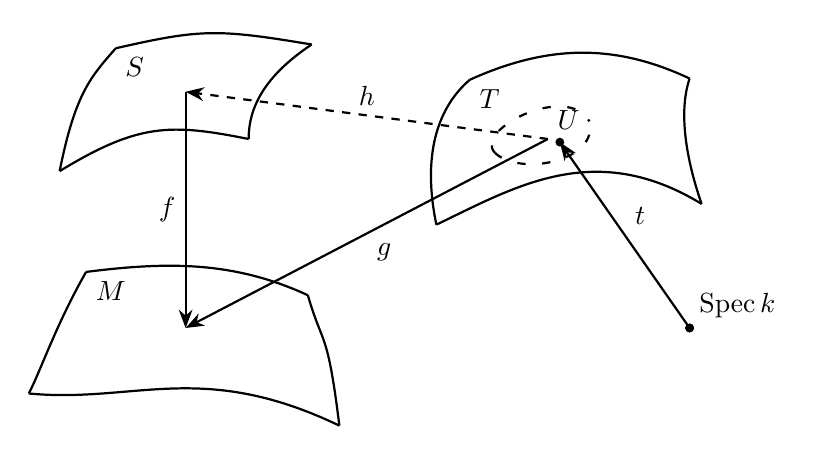
\begin{tikzpicture}[scale=0.8]
  % Coordinates
  \coordinate (A) at (-1.00, 5.99);
  \coordinate (B) at (-0.11, 7.94);
  \coordinate (C) at (-0.75, 7.24);
  \coordinate (D) at (-0.50, 7.49);
  \coordinate (E) at (3.00, 8.00);
  \coordinate (F) at (1.25, 8.25);
  \coordinate (G) at (1.50, 8.25);
  \coordinate (H) at (2.00, 6.50);
  \coordinate (I) at (0.25, 6.75);
  \coordinate (J) at (0.75, 6.75);
  \coordinate (K) at (2.00, 7.00);
  \coordinate (L) at (2.25, 7.50);
  \coordinate (M) at (4.98, 5.14);
  \coordinate (N) at (5.51, 7.44);
  \coordinate (O) at (4.75, 6.25);
  \coordinate (P) at (5.00, 7.00);
  \coordinate (Q) at (9.00, 7.46);
  \coordinate (R) at (6.75, 8.00);
  \coordinate (S) at (7.81, 8.02);
  \coordinate (T) at (9.19, 5.47);
  \coordinate (U) at (6.25, 5.75);
  \coordinate (V) at (7.50, 6.50);
  \coordinate (W) at (8.75, 6.75);
  \coordinate (X) at (8.96, 7.33);
  \coordinate (Y) at (-1.49, 2.46);
  \coordinate (Z) at (-0.58, 4.39);
  \coordinate (AA) at (-1.06, 3.55);
  \coordinate (AB) at (2.94, 4.02);
  \coordinate (AC) at (0.69, 4.55);
  \coordinate (AD) at (1.75, 4.57);
  \coordinate (AE) at (3.44, 1.95);
  \coordinate (AF) at (0.19, 2.30);
  \coordinate (AG) at (1.25, 3.00);
  \coordinate (AH) at (3.25, 3.50);
  \coordinate (AI) at (3.18, 3.19);
  \coordinate (AJ) at (-1.31, 2.80);
  \coordinate (AK) at (5.91, 6.28);
  \coordinate (AL) at (7.41, 6.78);
  \coordinate (AM) at (5.56, 6.65);
  \coordinate (AN) at (7.06, 7.40);
  \coordinate (AO) at (6.31, 5.90);
  \coordinate (AP) at (7.56, 6.15);
  \coordinate (AQ) at (6.75, 6.50);
  \coordinate (AR) at (1.00, 7.25);
  \coordinate (AS) at (1.00, 3.50);
  \coordinate (AT) at (9.00, 3.50);
  \coordinate (AU) at (6.94, 6.45);

  % Drawing
  \draw[thick] (A) .. controls (-0.75, 7.24) and (-0.50, 7.49) .. (B);
  \draw[thick] (B) .. controls (1.25, 8.25) and (1.50, 8.25) .. (E);
  \draw[thick] (A) .. controls (0.25, 6.75) and (0.75, 6.75) .. (H);
  \draw[thick] (H) .. controls (2.00, 7.00) and (2.25, 7.50) .. (E);
  \draw[thick] (M) .. controls (4.75, 6.25) and (5.00, 7.00) .. (N);
  \draw[thick] (N) .. controls (6.75, 8.00) and (7.81, 8.02) .. (Q);
  \draw[thick] (M) .. controls (6.25, 5.75) and (7.50, 6.50) .. (T);
  \draw[thick] (T) .. controls (8.75, 6.75) and (8.96, 7.33) .. (Q);
  \draw[thick] (Y) .. controls (-1.31, 2.80) and (-1.06, 3.55) .. (Z);
  \draw[thick] (Z) .. controls (0.69, 4.55) and (1.75, 4.57) .. (AB);
  \draw[thick] (Y) .. controls (0.19, 2.30) and (1.25, 3.00) .. (AE);
  \draw[thick] (AE) .. controls (3.25, 3.50) and (3.18, 3.19) .. (AB);
  \draw[loosely dashed,thick] (AK) .. controls (5.56, 6.65) and (7.06, 7.40) .. (AL);
  \draw[loosely dashed,thick] (AK) .. controls (6.31, 5.90) and (7.56, 6.15) .. (AL);
  \draw[-Stealth, dashed,thick] (AQ) -- node[above, text=black, midway] {$h$} (AR);
  \draw[-Stealth,thick] (AR) -- node[left, text=black, midway] {$f$} (AS);
  \draw[-Stealth,thick] (AQ) -- node[below right, text=black, midway] {$g$} (AS);
  \draw[-Stealth,thick] (AT) -- node[above right, text=black, midway] {$t$} (AU);
  \fill[black] (AT) circle (2pt);
  \fill[black] (AU) circle (2pt);
  \node[below right, black] at (B) {$S$};
  \node[below right, black] at (N) {$T$};
  \node[below right, black] at (Z) {$M$};
  \node[above right, black] at (AQ) {$U$};
  \fill[black] (AT) circle (2pt);
  \node[above right, black] at (AT) {$\Spec k$};
\end{tikzpicture}
\caption{局部万有性质}
\end{figure}


\subsection{代数群及其作用}

\begin{definition}[代数群作用]
  定义和定理等环境都可以输入标题. 在这个定义下面我们会插入并排的交换图.
  \upcite{EGAChinese1} 
\end{definition}

\begin{figure}[htbp]
  \centering
  \begin{minipage}[t]{0.45\textwidth}
    \centering
    \begin{tikzcd}
        \operatorname{Spec} k \times X 
        \arrow[r,"e \times \operatorname{id}_X"] 
        \arrow[dr,"\cong"'] 
        & G \times X 
        \arrow[d,"\sigma"] \\
        & X 
    \end{tikzcd}
    \caption{群作用的单位律}
  \end{minipage}
  \hspace{0.05\textwidth}  % 两张图之间留5%页面宽度的间距
  \begin{minipage}[t]{0.45\textwidth}
    \centering
    \begin{tikzcd}
        G \times G \times X 
        \arrow[r,"\operatorname{id}_G \times \sigma"] 
        \arrow[d,"m_G \times \operatorname{id}_X"'] 
        & G \times X \arrow[d,"\sigma"] \\
        G \times X \arrow[r,"\sigma"'] & X. 
    \end{tikzcd}
    \caption{群作用的结合律}
  \end{minipage}
\end{figure}

公式的输入和一般的一样. 

\begin{equation}
  \label{Eq1}
  \begin{aligned} 
    \varphi_{*}(f \cdot g)
    &= \varphi_{*}(m \circ (f \times g))\\
    &=  \varphi \circ m \circ (f\times g)\\
    &= m \circ (\varphi\times \varphi) \circ (f \times g)\\
    &= m \circ (\varphi f \times \varphi g)\\ 
    &= \varphi f \cdot \varphi g \\ 
    &= \varphi_{*}(f) \cdot \varphi_{*}(g).  
  \end{aligned}
\end{equation}

一般来说对公式的引用可以使用 \eqref{Eq1} 自动加上括号. 

\subsubsection{普通地插入图片}

\begin{figure}[htbp]
  \centering
  
\includegraphics[width=0.6\textwidth]{Peggy.jpg}
  \caption{巴猪猪来啦}
  \label{Fig1}
\end{figure}

我们也可以自动地引用图片, 图 \ref{Fig1}

\section{这里应该是你的第三章, 该开始推导了}

\begin{theorem}
  \label{Thm1} % 这里进行一个标注以引用, 如果不引用可以不用标注. 
  你会在这里列出你的主要定理. 
\end{theorem}

\begin{proof}
  然后在这里证明它. 
\end{proof}

一般来说定理的引用可以使用 \autoref{Thm1} 会自动加上环境的名称, 
但是由于我们为了方便定理的首行缩进, 直接采用了在定理前面加上空格这个操作, 
因此我们还是建议您自己手写, 定理\ref{Thm1}

如果你觉得定理环境你不喜欢, 比如说我在这里为了符合学校的要求, 
采取了统一字体和统一行间距的做法, 这其实大大牺牲了论文排版的美感, 
对此你可以回到 declaretheoremstyle 那里进行修改. 




\newpage
% ===================== 参考文献 =====================
\refstyle

\bibliography{reference.bib} % 插入参考文献列表, 索引的文件位置是同一个文件夹下的 reference.bib 文件

\newpage


\end{document}